\chapter{Evaluation}
\label{Evaluation}

Evaluation of a program like this is inherently difficult. There is no unified
agreement on exactly what is meant by program similarity. Other studies brush
over this fact as similarity is merely an intermediate value which is used 
to classify code as either plagiarised or not. As such, there are
issues with trying to get quantitative numerical results for a task like this,
and our evaluation primarily focuses on a qualitative approach.

Our data set included a number of Java coursework projects for around 120-
140 first year students, most learning Java for the first time. As such,
the test base represents our target population. Our research is aimed
at a tool to provide information to lab coordinators on their students'
exercises so it was an important data set to analyse.

\section{Algorithm findings}

We were able to generate some interesting cluster maps based on student exercises.
In Figures \ref{fig:recursionHeatmap}, (also seen in hierarchical only format in
\cref{fig:recursionHierarchy}) we can
see, in general, a couple of large clusters of student exercises, with weak
subclusters found amongst them. As well as this, we can see a few interesting
clusters and lack of them. Examining the three projects on the far right
of the map, these three cluster with each other, but quite loosely (indicated by
the purple colour of the relevant squares, and the hierarchy at the top).
Upon inspection of the code, we notice a difference immediately when compared
to other pieces of code for this exercise. These three users all answered this
exercise with an iterative solution; the name of the exercise was Java Recursion.
In this exercise, the students were expected to build their code recursively,
as the majority did, however these three students opted for a different style
and this is easy to pick up. The exercises which were implemented recursively
are still fairly weakly clustered when compared with the other clusters. This
is explained through their inconsistent use of loops -- the far right students
use many while and for loops (in differing numbers) compared with the other,
who only has a small smattering of while loops.


\begin{figure}

	\centering
		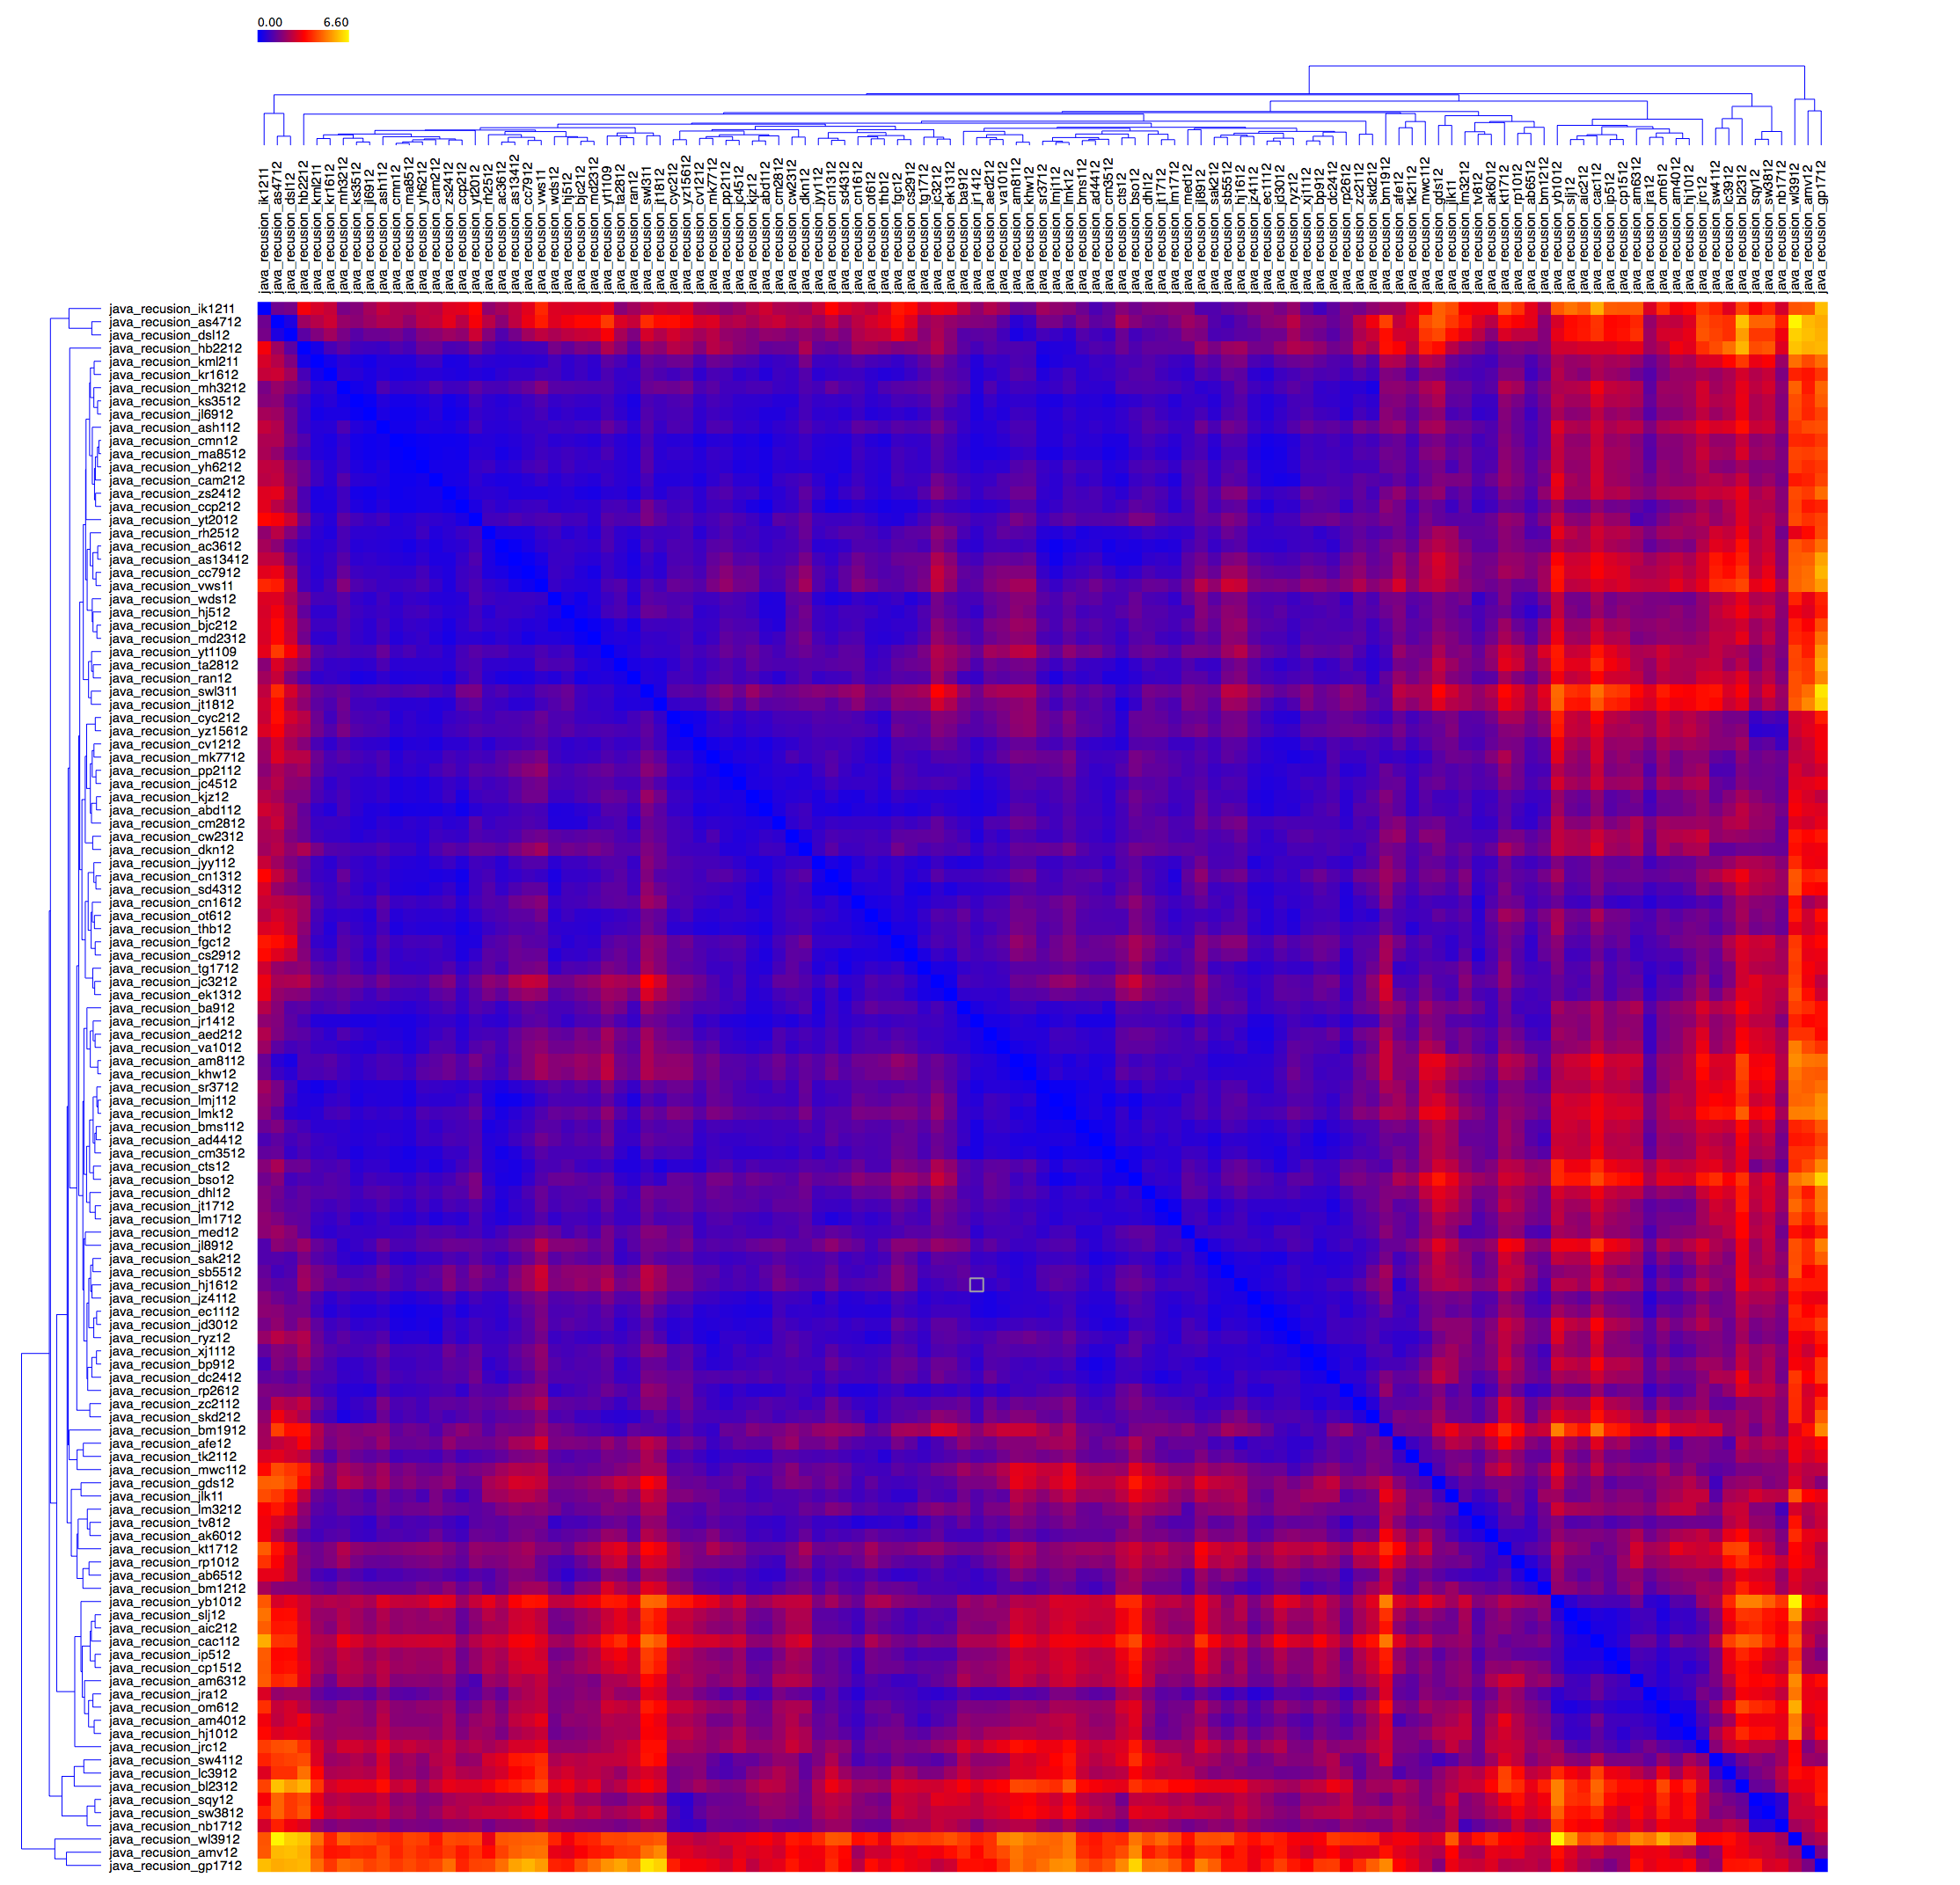
\includegraphics[width=1.2\textwidth]{Figures/RecursionHeatmap}
	\caption{A heatmap of similarities for a simple recursion exercise -- blue
	indicates high similarity, with red through green indicating lower
	similarities. \emph{Note: the usernames have been edited out of the map
	to preserve anonymity}}
	\label{fig:recursionHeatmap}

\end{figure}

Another observation from this heatmap is in the small two student cluster highlighted
in green. Upon opening the files together, we can see the two files are
plagiarised from one another \cref{code:recursionPlag}. We can see here that the
students have swapped the order of their method definitions, switched the
helper method's access modifier and renamed the helper method; the code however,
is almost identical. In the code segment below, our algorithm actually sees a
similarity of 1.0 (i.e. identical). The changes to method names, and the
reordering of \texttt{n == r} to \texttt{r == n} don't reduce similarity
as the id of these things is ignored; similarly, the \texttt{private} to 
\texttt{public} access modifier change is ignored. Finally, the order of the
method definitions has been swapped around, however due to the second improvement
to the parse tree kernel function \cpageref{secondImprovementParseTreeKernel}
the order of nodes doesn't matter, i.e. we can define our methods in any order
and the similarity will always be identical.

\begin{figure}[H]
\begin{minipage}[b]{0.45\linewidth}
\begin{lstlisting}[language=Java]

	public static boolean isHappy(int n) {
		return checkHappy(n, 0, 0, 0);
	}

	private static boolean checkHappy(int n, int r, int t, int nt) {
		if (n == 1) {
			return true;
		} else if (t > 0) {
			n = sumSquareDigits(n);
			t = t - 1;
			return checkHappy(n, r, t, nt);
		} else if (n == r) {
			return false;
		} else {
			n = sumSquareDigits(n);
			nt = nt + 1;
			t = nt;
			r = n;
			return checkHappy(n, r, t, nt);
		}

	}
\end{lstlisting}
\end{minipage}
\hspace{0.5cm}
\begin{minipage}[b]{0.45\linewidth}
\begin{lstlisting}[language=Java]

	public static boolean happy(int n, int r, int t, int nt) {
		if (n == 1) {
			return true;
		} else if (t > 0) {
			n = sumSquareDigits(n);
			t = t - 1;
			return happy(n, r, t, nt);
		} else if (r == n) {
			return false;
		} else {
			n = sumSquareDigits(n);
			nt = nt + 1;
			t = nt;
			r = n;
			return happy(n, r, t, nt);
		}
	}

	public static boolean isHappy(int n) {
		// TODO: Implement this method
		return happy(n, 0, 0, 0);
	}

\end{lstlisting}
\end{minipage}
\caption{Student solution to a section of Java Recursion coursework alongside
a clustered, high similarity piece}
\label{code:recursionPlag}
\end{figure}

When we extended our comparison to look at other nodes in the cluster, we found
that the submission immediately to the right of the highlighted area was also
a plagiarised submission of the same files. The similarity was less pronounced
as this student had avoided some of the tasks, reducing the score.

The Hierarchical Clustering node has been configured to show a reasonable number
of submissions per cluster. What is defined as ``reasonable'' is open to debate,
however we can start to see similar patterns emerging from the defined clusters.
Interestingly there also appears to be a distinction between clusters too --
the problem of identifying differences in code is perhaps even more difficult
than identfying similarities. Still, given the example of an iterative solution
to recursive exercise, and the reluctance of that cluster to combine with others,
it is a good indication of validity.

Our succesful cases aren't constrained to the one exercise either. 
\cref{fig:LoopsAndArraysHeatmap} and \cref{fig:LoopsAndArraysHierarchy}
demonstrate the outputs of our similarity function to the parse tree kernel
function.

Our implementation has proven to be successful in identifying a number of
interesting findings in our code bases. Unfortunately, it is not as successful
in every instance. If we take a more complex coursework, such as Discrete
Event Simulation, and run the same tests, our output is not as useful. 
\cref{fig:DESHeatmap} shows the heatmap we generate from this data set. The
yellow colour is used to indicate the maximum distance value of the graph. Here,
the maximum value is 100, indicating an overflow of similarity (i.e. the algorithm
return $N(s, s') > 1$). If we receive an result greater than one, there is no
indication of what really this means. According to \cite{ParseTreeKernel},
the normalisation of the kernel function should guarantee a value between 0
and 1. After much debugging of our code, we decided to investigate this claim
of similarity bounds. 

Consider the parse trees given in \cref{fig:OverflowParseTreesBeforeReflex}
Before 

\begin{figure}[H]

	\centering
		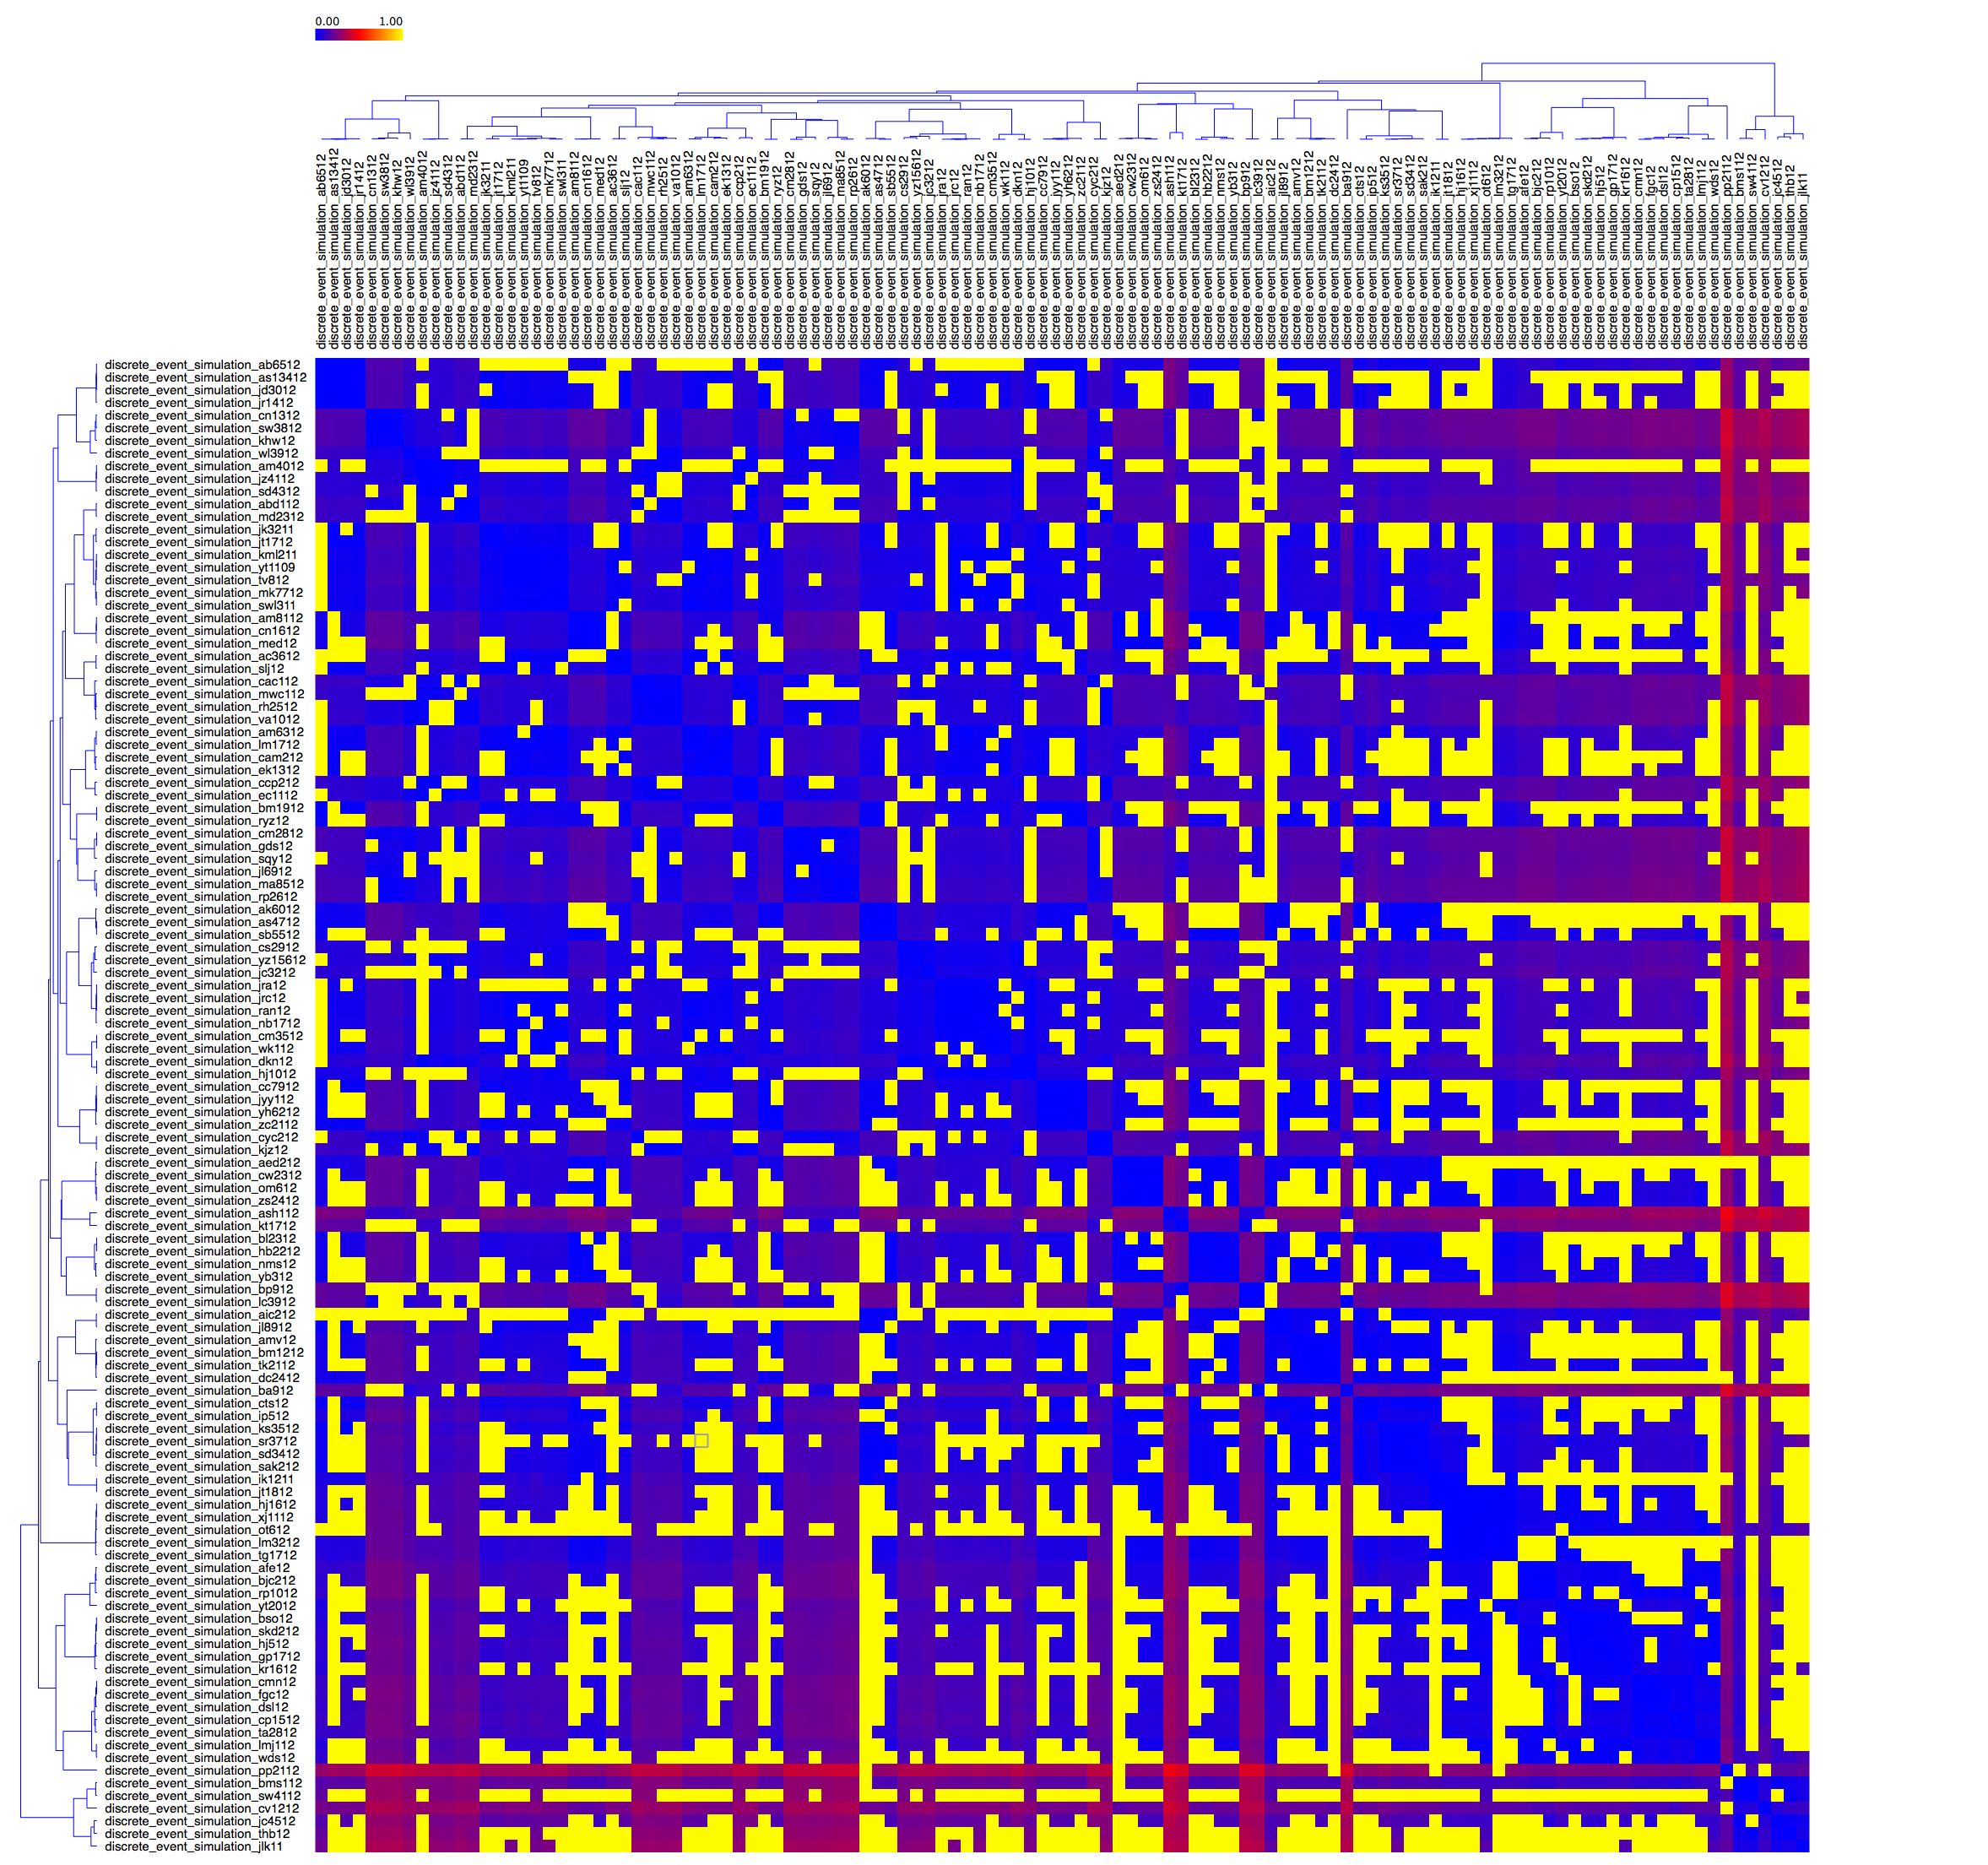
\includegraphics[width=1.2\textwidth]{Figures/DESHeatmapOverflow}
	\caption{Discrete Event Simulation Heatmap}
	\label{fig:DESHeatmap}

\end{figure}

\section{Reflexivity}
In a similarity measure, we expect the output to be reflexive, that is the similarity of trees `A' and `B' should be equal to the similarity of trees `B' and `A'. The algorithm doesn’t actually address this issue, and in its original state, it is not reflexive.

For example take the parse trees in ??. If we apply the C step of the parse tree kernel algorithm to the root nodes of T1 and T2(i.e. 
$C(ClassDefinition\textsubscript{T1},ClassDefinition\textsubscript{T2}$) assuming a decay factor of $\lambda$ and $threshold depth > 1$, we get the result $\lambda(1 + \lambda)$. 
We get this result as the comparison of root nodes yields 
$lambda \times x$ where $x$ is the result of the product of the similarity of T1s children
with T2s children (the $\prod_{i}^{nc(n\textsubscript{1})}{(...)}$ part in the algorithm). 
As the root of T1 only has one child, $x$ evaluates to
$1 + C(MethodDeclaration\textsubscript{T1}, MethodDeclaration\textsubscript{T2})$. Note that as both
children in T2 are the same type, we will get the same result. Here we reach
a base case of C as both nodes are terminals, and return $\lambda$.

Conversely, if we calculate the reverse, 
$C(ClassDefinition\textsubscript{T2}, ClassDefinition\textsubscript{T1})$, using the same constants, we get the result $\lambda(1+\lambda)^2$. As above the comparison of the root nodes yields $\lambda \times x$. This time, when calculating $x$, we must
iterate over both child nodes in T2, comparing it with the single child node of
T1. Each node comparison multiplies the result by $1+C(MethodDeclaration\textsubscript{T2},MethodDeclaration\textsubscript{T1})$, the call to $C$ returning $\lambda$, as above. As such, we have a different result depending on the order of comparison.
The options we had in modifying the algorithm to maintain reflexivity
\todo{parse trees that aren’t reflexive}

focussed on the fact that regardless of order the nodes were passed in to the comparison function, the children must be iterated on in the same manner. 
\todo{could have iterated both ways and taken an average, copmutationally infeasible}
i.e. if $C(n\textsubscript{1},n\textsubscript{2})$ goes through each child of $n\textsubscript{2}$ and the max similarity of each with $n\textsubscript{1}$, then the same should happen for
$C(n\textsubscript{2},n\textsubscript{1})$. We could have calculated the hashcode of the inputted node and then chosen, for example, the node with the smallest hashcode to be the `primary' iterated node. This, however, is an arbitrary decision and doesn’t address the issue of why we get different values for similarity. The decision was to check the number of children of the two root nodes, and make the node with the fewest number of children the primary node.
This decision is justified in the context. Consider a modified version of the two trees in 
\cref{fig:nonReflexTree}, where T\textsubscript{2} has a large number of method declarations, asin \cref{fig:manyMethodTree }and T\textsubscript{1} remains the same. If we set the
root of T\textsubscript{2} to be the primary node, we would match every child node with the one child node of T\textsubscript{1}, artificially inflating the similarity between the two, when the similarity it could be argued, is actually much smaller. Rather, it is more useful to set the root of T\textsubscript{1} as the primary node -- this will match the child node once with any child of T\textsubscript{2}, but only once. Once the normalising step is applied, the size of 
T\textsubscript{2} is likely to reduce the effect this matched node has as the unnormalised similarity of T\textsubscript{2} with itself will be much greater than that of the two trees’ unnormalised similarity with each other. 

This method of ordering takes care of most cases of reflexivity, but it
was discovered that non-reflexive results could still occur in the instance de-
scribed in \ref{fig:furtherNonReflex}. Here, the two trees have the same number of children, so the
previous problem is avoided, however it is a case that has been previously
missed. If the roots of trees T\textsubscript{1} and T\textsubscript{2} are passed in
 to $C(n\textsubscript{1},n\textsubscript{2})$, there
is no guarantee that the outcome will be the same when the arguments are reversed. With the above example, in calculating $C(ClassDefinition\textsubscript{T\textsubscript{1}},ClassDefinition\textsubscript{T\textsubscript{2}})$, we would set the first argument as the primary node. Iterating over the
children of this node, and comparing them with all nodes of the second argument, 
we get the result $\lambda(1 + 0)(1 + \lambda)$. This occurs because the Modifier
child node doesn’t match with any of the children of T\textsubscript{2}, and the recursive
call hits the base case for different $n\textsubscript{1}$ and $n\textsubscript{2}$ (i.e. return 0) in each 
comparison. Swapping the order of the arguments results in the root of T\textsubscript{2} being the
primary node. As we use the maximum value returned for the comparison
of each child node, the two MethodDeclaration nodes both match with the one MethodDeclaration node in T1, thus the result of the similarity comparison is $\lambda(1 + \lambda)^2$.

Again, we have multiple methods with which to overcome this issue and ensure reflexivity. Our approach looked at the uniqueness property of the children. If a single node has many child nodes of mostly similar types, and is compared with a node which has many unique type of child nodes, it is likely that the children of the unique style node contain at least one node that the non-unique children of the first node can all match with. i.e. a node, n\textsubscript{1}, with 5 MethodDeclaration children and a node, n2, with 1 MethodDeclaration child and 4 assorted children (e.g. Modifier, FieldDeclaration etc.), if compared with n\textsubscript{1} as the primary node, would return $\lambda(1 + \lambda)^5$ -- a high value -- even though only one node was similar. We also see no reference to the dissimilar nodes in the similarity score. Instead, we set the primary node to be the node with the most uniquely typed children, ensuring that a node with many different type of child nodes will match only partially against a node with identical children.
If the uniqueness value is the same for both nodes, it is still possible that the children are different. In this case, we use a priority queue, adding the the children to the queue, with one queue for each root node. These queues are then iterated over and once a mismatch is found in the elements at the same index, the node whose queue has the highest priority at this index is chosen as the primary node. This is an arbitrary decision and could be improved upon further, however
the extension involves a substantial amount of work for only a small gain in correctness in a
very rare edge case.

If this situation were to occur, we could ideally have a priority queue of all
node types, with the more important types at the front, and the least important
at the end. For example, a \texttt{do...while} block could be considered higher
priority as they are more rare; this queue would be iterated through and the 
node with the highest priority unique child would be set as the primary. As stated,
this would take a lot of effort, weighing up the value behind each type of node
of the parse tree, of which there are around 100, so this was left unimplemented.

\todo{fails when smaller tree is duplicated numerous times in bigger tree}


\subsection{Heuristic choices}
The heuristic choices, \emph{threshold depth} and \emph{decay factor}, were 
set as 3 and 0.3 in the initial research for the algorithm\cite{ParseTreeKernel}. 
The paper doesn't offer any insight as to how to calculate the optimal values
for this so we developed our own technique. We noticed that generally a higher value
for each would incorporate more information in a similarity analysis. Although we
want to avoid the issues discussed in \cref{Background} where the root node has
an overwhelming effect on the score, a tree with matching nodes that goes down
many levels should contribute to the score more, as this kind of structure matching
is very unlikely and thus indicitave of similar code, justifying increasing the
threshold depth somewhat. Also for the decay factor, a deep matching tree is
very useful in identfying similar segments.

Ideally in setting these parameters, we want to find a balance between values
high enough to provide the most insight, but low enough so as not to imbalance
the score as described previously. To calculate this value, we branched off
from our main commit branch and generated some tests to calculate the similarity
scores with every combination of $decay factor=[0.05, 0.1 .. 0.25, 0.3, 0.4 .. 0.9, 1.0]$
and $threshold depth=[1, 2 .. 10]$. Our initial plan was to see how the heatmaps
looked with each combination of heuristics, eliminating any that combinations
that were plainly wrong, e.g. giving too many very low or very high similarity
values/combinations which didn't allow much to distinguish between projects.
Upon running the algorithm however, we encountered the overflow problem discussed
in \cref{sec:Overflow}. This led to a limited number of combinations we could use.
The maximum \emph{threshold depth} we could consistently use was 3, and similarly for
a \emph{decay factor} of 0.2. As this maximum was less than even the suggested values,
we opted to keep these values.

\subsection{Result Dimensionality}
\label{sec:VisTech}
Orange provides a wide variety of visualisation tools for analysis, however,
for most of these, expects an array of feature vectors to be passed in, with
Orange generating the distances itself. Using the distances and the original
values, it is able to display a large number of information types. It would be
ideal if we could utilise some of these extra tools for our analysis. Specifically,
an issue with our clustering method, is that it is confined to the single dimension.
There are a few times throughout the maps where we see small parts of a cluster
that acutally have high similarity with other clusters (to find these 
additional clusters, we need to look for larger squares of similarity away from
the main diagonal). This indicates that, although the cluster this subcluster
is part of is the most appropriate, it could also belong to the other cluster,
where the rest of the nodes in the original cluster may not belong. Seen in
\cref{fig:NonClusteredCluster}, the squares highlighted in green could be part
of both the black cluster, which it currently is, as well as the white cluster,
whilst the rest of the black cluster shouldn't be linked with it. 

A network graph could be a perfect way to demonstrate this, with nodes connected
to other nodes with which it shares a similarity above a certain threshold,
arranging this network could help highlight added regions. These regions could
occur where parts of a project, perhaps the first half of an exercise, were
completed in a certain way by a group of students. A subset may have completed
the second half in a way that is unique from the rest of the set, but similar
to how yeat another group of students completed it. This would be great to
highlight to lab coordinators, who could provide group feedback on a per method
basis for example.

\section{File Compare View}
The protoype compare view is an 

\todo{hard to evaluate}
\todo{predictive validity}
\todo{different sized trees dont work very well -- DSE as an example}
\todo{simplistic code, ok for our purpose. genrealisable to bigger projects?}
\todo{where it falls down}
\todo{speed}
\todo{unable to reproduce results}
todo[integration of other algos]

todo[file compare view: needs improving]

todo[file compare view: is it right?]